\appendix
\section{Experiment Details}

\subsection{Resource Cost}
The cost of tool calls is determined by the pricing of the providers. 
To standardize billing, we've established a unified rate of \$0.001 per invocation for both search API calls and web browsing actions. 
Because different URLs produce varying amounts of text and tokens, this per-call rate is derived as an average computed from post hoc statistics over all our experiments.
The consumption of tokens is billed separately, adhering to the official pricing models of the API provider pricing\footnote{\url{https://cloud.google.com/vertex-ai/generative-ai/pricing}}.




\subsection{Implementation Details}
To keep the context length manageable, we employ several simple context management strategies. For each browse tool call, the fetched webpage is truncated to 150,000 characters before being sent to the model. At every iteration, we discard tool outputs from previous steps and retain only the most recent tool response, preventing the context from growing with accumulated tool results. 
In \method's verification module, we further control context size by periodically replacing the historical trajectory with summary. Since the agent determines when to activate the verification module, we perform a check during each invocation: if more than $K$ iterations have passed since the last update (with $K=10$ in our experiments), we replace the older reasoning trace with a concise summary derived from the verification outputs.







\section{Additional Analysis}

\subsection{Tool Usage}\label{app:usage_breakdown}

\begin{table}[h]
\centering
\caption{Resource usage statistics of the ReAct baseline using Gemini-2.5-Pro and Gemini-2.5-Flash on the BrowseComp dataset. Over-Budget \% denotes the percentage of data that reaches the given tool budget limit.}
\label{tab:react_budget_usage}
\small
\begin{tabular}{lrrrrrr}
\toprule
\multirow{2}{*}{\textbf{Model}} &
\multirow{2}{*}{\textbf{Budget}} &
\multirow{2}{*}{\textbf{Acc \%}} &
\multicolumn{2}{c}{\textbf{Query}} &
\multicolumn{2}{c}{\textbf{URL}} \\
\cmidrule(lr){4-5} \cmidrule(lr){6-7}
& & & \textbf{Avg. \#} & \textbf{Over-Budget \%} 
  & \textbf{Avg. \#} & \textbf{Over-Budget \%} \\
\midrule

% ====================== Pro ======================
\multirow{3}{*}{Gemini-2.5-Pro}
& 30  & 10.5 & 13.77 & 9.24   & 1.33 & 0.00 \\
& 50  & 12.4 & 13.95 & 0.79   & 1.31 & 0.00 \\
& 100 & 12.6 & 14.24 & 0.00   & 1.36 & 0.00 \\

\midrule

% ====================== Flash ======================
\multirow{3}{*}{Gemini-2.5-Flash}
& 30  & 9.0  & 22.77  & 42.81  & 1.04 & 0.00 \\
& 50  & 9.7 & 28.88 & 14.22  & 1.24 & 0.00 \\
& 100 & 10.0 & 29.93 & 2.6   & 1.36 & 0.00 \\

\bottomrule
\end{tabular}
\end{table}

In Table~\ref{tab:react_budget_usage}, we examine how the ReAct baseline utilizes tools under different budget constraints on the BrowseComp dataset. As expected, increasing the allowed tool budget enables the agent to interact more with the environment, leading to improved accuracy. The Over-Budget\% column shows the proportion of examples that exhaust the allocated tool budget. For Gemini-2.5-Pro, only 0.8\% of the data requires more than 50 tool calls, whereas Gemini-2.5-Flash shows a higher reliance on tool usage, with 2.6\% of the queries exceeding a budget of 100. Notably, Flash models issue roughly twice as many search queries as Pro models. This suggests that the stronger parametric knowledge of Gemini-2.5-Pro allows it to navigate the search space more efficiently, reducing reliance on externally gathered evidence and enabling it to solve queries with fewer tool calls.

\subsection{Details of Parallel Scaling}\label{app:pass@n}

For Majority Vote, we aggregate the final answers across different samples and use a judge model (Gemini-2.5-Flash) to identify the consensus answer. For Best-of-N, we provide all response trajectories to the judge model and select the most promising one. For Pass@N, the score is calculated as 1 if any of the sampled responses contain the correct answer.
The prompts used for these evaluations are provided in Appendix~\ref{app:prompt_answer}.
In Figure~\ref{fig:bt_parallel_pass}, we additionally report the Pass@N results for ReAct and Budget Tracker under parallel scaling settings. Budget Tracker consistently achieves higher overall accuracy across varying budgets and cost levels.

\begin{figure}[h]
    \centering
    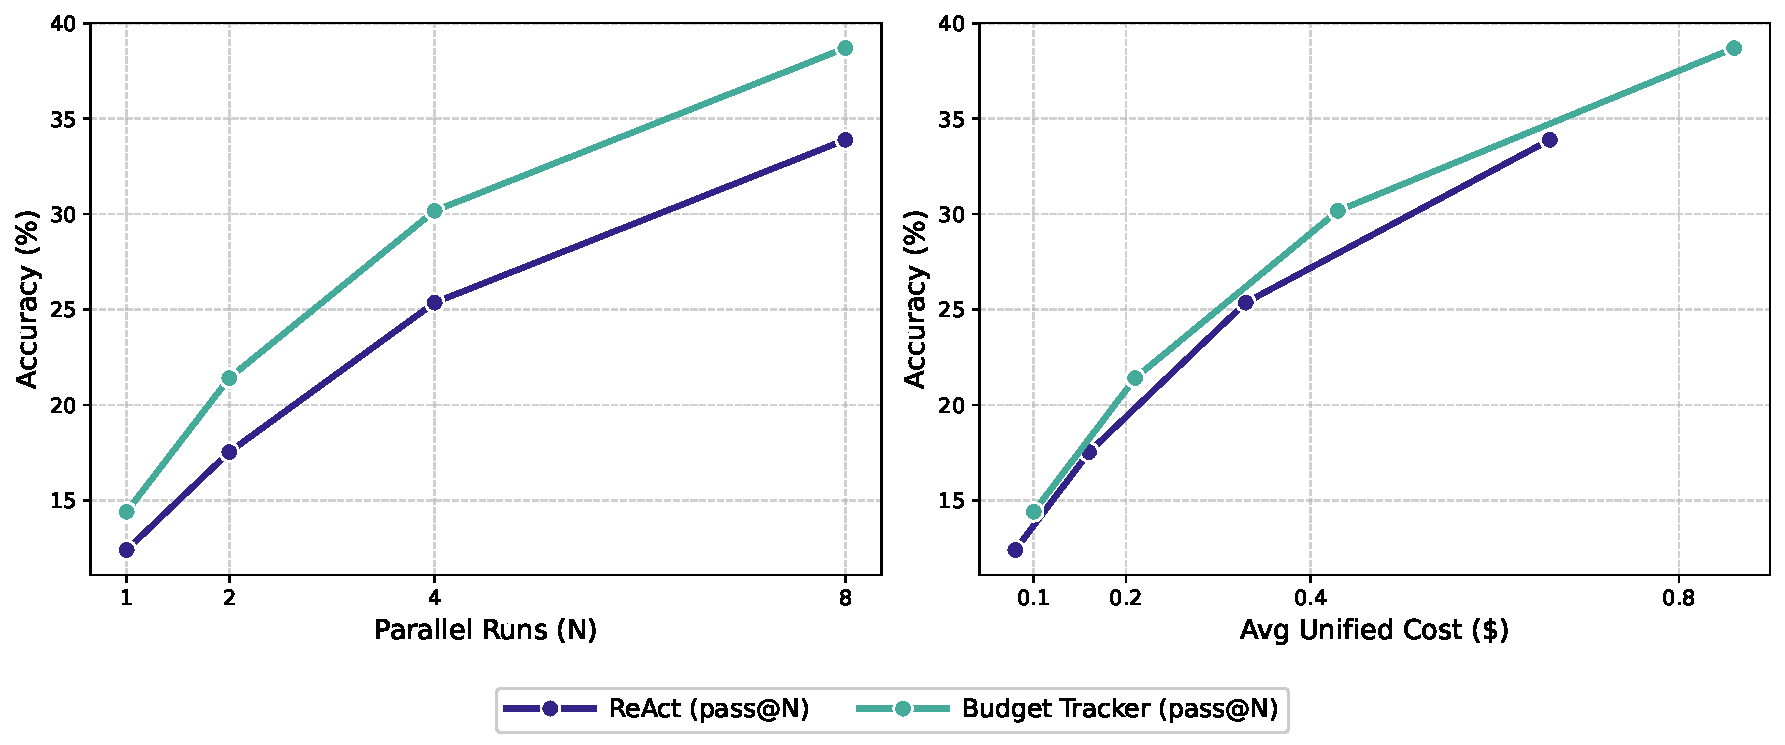
\includegraphics[width=0.85\linewidth]{assets/figs/bt_parallel_pass.pdf}
    \caption{Pass@N results of Budget Tracker and ReAct in parallel scaling. 
The left subfigure shows accuracy scaling with increasing parallel runs, 
while the right subfigure illustrates the corresponding cost–performance trend.
    }
    \label{fig:bt_parallel_pass}
\end{figure}


\subsection{Resource Usage}


Table~\ref{tab:resource_detail} reports the detailed breakdown of tool calls and token consumption in \method using Gemini-2.5-Pro on BrowseComp. We compare our approach against the variant \method-response, which keeps the full tool responses from previous rounds. In contrast, \method removes these responses to optimize context length.
In the table, token usage is reported as a triplet: (Input / Output / Cache). The results demonstrate that removing historical tool responses does not compromise performance (maintaining similar accuracy) but significantly reduces computational overhead. This efficiency is evidenced by the substantial decrease in cache tokens and the reduction in overall cost.

\begin{table}[h]
    \centering
    \caption{Resource usage comparison. Token counts are reported as Input / Output / Cache (in 10,000). ``Veri. tokens'' denotes the usage of the self-verification module. \method achieves comparable accuracy to the full-context baseline (\method-response) while significantly reducing cache token usage and unified cost.}
    \label{tab:resource_detail}
    \begin{tabular}{lcccccc}
        \toprule
        & \textbf{Acc (\%)} & \textbf{\# search} &\textbf{\# browse} & \textbf{Total tokens} & \textbf{Veri. tokens} & \textbf{Cost (\$)} \\
        \midrule
        BATS & 24.6 & 87.3 & 13.6 & 32.1 / 6.9 / 39.3 & 1.1 / 1.2 / 7.6 & 1.1 \\
        BATS-response & 24.3 & 84.4 & 14.6 & 33.6 / 6.5 / 91.8 & 1.0 / 1.3 / 17.1 & 1.2 \\
        \bottomrule
    \end{tabular}
\end{table}





\subsection{Early Stopping}

\begin{wrapfigure}{r}{0.5\textwidth}  
  \centering
  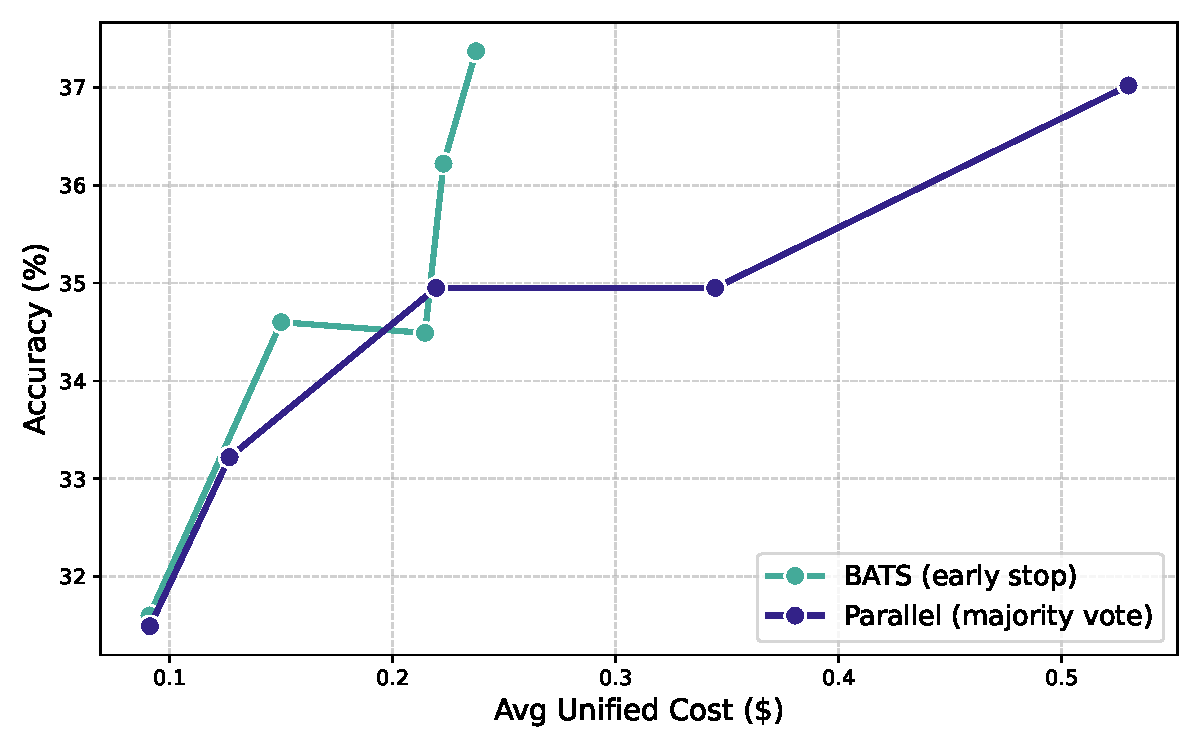
\includegraphics[width=0.98\linewidth]{assets/figs/first-bczh-pro-cost.pdf}
  \caption{Average unified cost analysis on BrowseComp-ZH using Gemini-2.5-Pro.}
  \label{fig:first-bczh-cost}
\end{wrapfigure}


\textbf{\method pushes the cost–performance Pareto frontier even further by leveraging early stopping.}
To provide a direct and transparent comparison of cost-efficiency, Figure~\ref{fig:first-bczh-cost} shows accuracy against the actual unified cost. \method demonstrates a much steeper performance curve, indicating that it achieves higher accuracy for a lower cost compared to the parallel majority vote baseline. \method reaches over 37\% accuracy for approximately \$0.23, while the parallel baseline requires more than double that cost (over \$0.50) to achieve a comparable result. The slight fluctuation is due to the small size of the BrowseComp-ZH dataset.
This efficiency benefits from its budget-aware verification module, which enables early termination upon finding a satisfactory answer and minimizes unnecessary spending.

\subsection{Planning Module}\label{app:early}
To evaluate the impact of the planning module, we augment the ReAct baseline with our proposed design, which integrates constraint analysis and a dynamically structured checklist plan. The tool-call budget is capped at 200 for both search queries and browse URLs. As shown by the Gemini-2.5-Pro results in Table~\ref{tab:abl_plan}, the addition of planning module alone improves the agent’s ability to organize exploration and utilize tool usage more effectively, resulting in a performance gain of 1.8\%. 

\begin{table}[h]
\centering
\caption{Effect of the planning module. With the same budget, the planning module encourages better  and yields higher average performance.}
\begin{tabular}{lrrr}
\toprule
\textbf{Method} & \textbf{Acc \%} & \textbf{Avg. \# Query} & \textbf{Avg. \# URL} \\
\midrule
ReAct & 11.0 & 7.75 & 0.35 \\
ReAct + planning & 12.8 & 13.81 & 0.82 \\
\bottomrule
\end{tabular}
\label{tab:abl_plan}
\end{table}





\lstdefinestyle{boxedcode}{
  basicstyle=\ttfamily\scriptsize,
  columns=fullflexible,
  keepspaces=true,
  breaklines=true,
  upquote=true,
  lineskip=-1pt
}




\section{Prompts}\label{app:prompts}

Our prompt for web search agents is developed based on \citet{DBLP:journals/corr/abs-2503-09516} and \citet{DBLP:journals/corr/abs-2507-02592}.

\subsection{ReAct+ Budget Tracker}\label{app:prompt_budget}

\begin{center} % 仅用于整体居中（可选）
\begin{tcolorbox}[
  enhanced,
  breakable,                 % 允许跨页
  colback=white,
  colframe=black!50!white,
  title={ReAct + Budget Tracker},
  width=1.0\linewidth        % 控制盒子宽度
]
\lstset{style=boxedcode}
\begin{lstlisting}
You are an AI reasoner with Google Search and Browsing tools. Solve the question by iterating: think, tool_code, tool_response, answer.

## Tools
You have access to 2 tools: search and browse.
{
  "name": "search",
  "description": "Performs batched web searches: supply an array 'query'; the tool retrieves the top 10 results for each query in one call.",
  "parameters": {
    "type": "object",
    "properties": {
      "query": {
        "type": "array",
        "items": {
          "type": "string"
        },
        "description": "Array of query strings. Include multiple complementary search queries in a single call."
      }
    },
    "required": [
      "query"
    ]
    }
},
{
  "name": "browse",
    "description": "Visit webpage(s) and return the summary of the content.",
    "parameters": {
        "type": "object",
        "properties": {
            "url": {
                "type": "array",
                "items": {"type": "string"},
                "description": "The URL(s) of the webpage(s) to visit. Can be a single URL or an array of URLs."
            },
            "goal": {
                "type": "string",
                "description": "The specific information goal for browsing webpage(s)."
            }
        },
        "required": [
            "url",
            "goal"
        ]
    }
}

You should start with one or more cycles of (thinking about which tool to use -> performing tool code -> waiting for tool response), and end with (thinking about the answer -> answer of the question). The thinking processes, tool codes, tool responses, and answer are enclosed within their tags. There could be multiple thinking processes, tool codes, tool call parameters and tool response parameters.

## Budget

You have two independent budgets:
- Query Budget (for search)
- URL Budget (for browse)
Each string in 'query' or 'url' consumes 1 unit respectively.

After each <tool_response>, a <budget> tag shows remaining units.
You must ADAPT your strategy dynamically to the current budget state.

### HIGH Budget (>=70% remaining)
- Search: 3-5 diverse queries in one batch.
- Browse: up to 2-3 high-value URLs.
- Goal: Broad exploration, build context fast.

### MEDIUM Budget (30%-70%)
- Search: 2-3 precise, refined queries per cycle.
- Browse: 1-2 URLs that close key knowledge gaps.
- Goal: Converge; eliminate uncertainty efficiently.

### LOW Budget (10%-30%)
- Search: 1 tightly focused query.
- Browse: at most 1 most promising URL.
- Goal: Verify a single critical fact or finalize answer.

### CRITICAL (<10% remaining or 0 in one budget)
- Avoid using the depleted tool.
- Only perform 1 minimal-cost query or browse if absolutely essential.
- If uncertainty remains and no tool use is possible, output <answer>None</answer>.

## Step syntax

<think>
Thinking process. Analyze the query, your internal knowledge, and search results to build your reasoning. Always justify tool choices based on the remaining budgets.
</think>
<tool_code>
{"name": "tool name here", "arguments": {"parameter name here": parameter value here, "another parameter name here": another parameter value here, ...}}
</tool_code>
<tool_response>
tool_response here
</tool_response>
<budget>
Query Budget Used: [number], Query Budget Remaining: [number], URL Budget Used: [number], URL Budget Remaining: [number]
</budget>

Repeat <think><tool_code> until you have the final answer.
<answer> Final solution only. </answer> 

## About answers

* Only write the final answer inside <answer> and </answer>.
* If you cannot find the answer, write <answer>None</answer>.
\end{lstlisting}
\end{tcolorbox}
\captionsetup{justification=centering} 
\captionof{figure}{Prompts used in ReAct + Budget Tracker.}
\label{fig:prompt_plan}
\end{center}



\subsection{Planning Module}\label{app:prompt_plan}

\begin{center} % 仅用于整体居中（可选）
\begin{tcolorbox}[
  enhanced,
  breakable,                 % 允许跨页
  colback=white,
  colframe=black!50!white,
  title={Budget-aware Planning Module in BATS},
  width=1.0\linewidth        % 控制盒子宽度
]
\lstset{style=boxedcode}
\begin{lstlisting}
## About questions

Questions contain two types of constraints: exploration and verification. 
* Exploration: Broad, core requirements (e.g., birthday, profession). Use these for initial searches to surface candidates. You may combine 1-2 to form stronger queries.
* Verification: Narrow, specific details. Apply these only after you have candidates, to confirm or filter them. Never begin with verification constraints.
Start with exploration queries, then use verification to validate the results.

## About planning

Maintain a tree-structured checklist of actionable steps (each may require several tool calls).
- Mark each step with its status: [ ] pending, [x] done, [!] failed, [~] partial.
- Use numbered branches (1.1, 1.2) to represent alternative paths or candidate leads.
- Log resource usage after execution: (Query=#, URL=#).
- Keep all executed steps, never delete them, retain history to avoid repeats.
- Update dynamically as you reason and gather info, adding or revising steps as needed.
- Always consider current and remaining budget when updating the plan.
\end{lstlisting}
\end{tcolorbox}
\captionsetup{justification=centering} % 可选：让标题居中
\captionof{figure}{Prompts used in planning module of BATS.}
\label{fig:prompt_plan}
\end{center}


\subsection{Self-verification Module}\label{app:prompt_verification}

\begin{center} % 仅用于整体居中（可选）
\begin{tcolorbox}[
  enhanced,
  breakable,                 % 允许跨页
  colback=white,
  colframe=black!50!white,
  title={Budget-aware Self-verification Module in BATS},
  width=1.0\linewidth        % 控制盒子宽度
]
\lstset{style=boxedcode}
\begin{lstlisting}
You are an AI Strategic Verifier. Your primary goal is to evaluate a proposed answer, assess the viability of the current problem-solving plan, and decide the best course of action: declare success, continue with the current plan, or pivot to a new one.

### Given Inputs

* Question: The original user question. An answer is believed to exist.
* Trajectory: The sequence of reasoning steps and tool calls taken so far in the current attempt.
* Current Answer: The final answer produced by the current attempt.
* Budget Status: Information on current tool call budget utilization and remaining budget, including search queries and browsing urls.

### Your Task: A 3-Step Process

You must proceed in the following order:

#### Step 1: Conduct Verification Analysis

First, perform a strict verification of the `Current Answer`.
* Go through each constraint from the original Question one by one.
* For each constraint, compare it against the `Current Answer` and the `Trajectory`.
* State your finding for each constraint: satisfied, contradicted, or unverifiable.

#### Step 2: Make a Strategic Decision

Based on your verification and the budget, make one of three decisions.

1. SUCCESS: If the verification in Step 1 passed (all constraints are satisfied). The task is complete.
2. CONTINUE: If the verification failed because few constraints are unverifiable, but the overall plan is still sound and salvageable. This is the choice if **both** of these conditions are true:
    * Promising Path: The `Trajectory` is generally sound, and the failure was due to a correctable error.
    * Sufficient Budget: There is enough `Remaining Budget` to attempt a correction on this path.
3. PIVOT: If the verification failed, signal to abandon the current plan and switch to another one. You should pivot if any of these conditions are true:
    * Dead End: The `Trajectory` reveals a fundamental flaw in the current plan's logic that cannot be easily fixed.
    * Failed Tool Calls: The Trajectory shows repeated, unsuccessful attempts to find certain info.
    * Insufficient Budget: The `Remaining Budget` is too low to make another meaningful attempt or correction within the *current* plan.

#### Step 3: Summarize for the Next Step

This is the most critical step for guiding future actions. 
You need to first provide a **trajectory summary**: Summarize the agent's reasoning trajectory into a concise narrative. Explain its initial goal, the logical steps taken, key findings and the final conclusion, emphasizing how key findings or contradictions caused the agent to change its strategy.

Then, provide additional details tailored to your decision in Step 2.

* If the decision is SUCCESS:
    * No further detail needed.

* If the decision is CONTINUE / PIVOT:
    * Failure Analysis: Diagnose the root cause of the failure. Identify the critical flaw (e.g., poor query design, flawed logic, misinterpreted evidence) and name the general failure pattern to prevent its recurrence.
    * Useful information: Any useful intermediate findings or results from the current `Trajectory` that could be valuable inputs for the next attempt. This prevents redundant work.
    * Strategic Recommendations: Provide actionable advice for the agent's next attempt. Suggest strategic pivots, new angles of investigation, or different ways to combine the problem's constraints. Explicitly state if it should backtrack to and resume from a specific step in the previous plan to avoid re-doing work.

### **Output Requirement**

Your final output must be a single JSON object with the following structure. Do not add any text before or after this JSON block.

```json
{
  "verification": "Verification analysis",
  "decision": "SUCCESS | CONTINUE | PIVOT",
  "justification": "A concise explanation for your strategic decision. Why is it a success, a dead end, or a correctable error?",
  "trajectory_summary": "The informative trajectory summary.",
  "details": "A JSON object containing the additional details required by Step 3. For a SUCCESS decision, this can be an empty object {}."
}
```
\end{lstlisting}
\end{tcolorbox}
\captionsetup{justification=centering} % 可选：让标题居中
\captionof{figure}{Prompts used in self-verification module of BATS.}
\label{fig:prompt_verification}
\end{center}


\subsection{Answer Selection}\label{app:prompt_answer}

\begin{center} % 仅用于整体居中（可选）
\begin{tcolorbox}[
  enhanced,
  breakable,                 % 允许跨页
  colback=white,
  colframe=black!50!white,
  title={Best-of-N Answer Selection},
  width=1.0\linewidth        % 控制盒子宽度
]
\lstset{style=boxedcode}
\begin{lstlisting}
You are an expert evaluator. Your task is to select the most accurate and specific answer to an information-seeking question. The question has a deterministic answer. You'll be provided with several answers and their corresponding trajectories/verifications.

**Instructions:**
1.  **Identify the Core Question:** Determine the exact piece of information the question is asking for (e.g., a person, a location, a date).
2.  **Evaluate Candidates:** For each candidate phrase, assess its factual accuracy.
3.  **Compare and Select:** Choose the answer that is more likely to be correct. You should never choose "None" as the answer.

**Output Format:**
First, provide a brief justification explaining why the chosen answer is the most accurate and specific choice. Then, on a new line, output the letter of the best option inside a box.

**Example:**
Justification: Answer B is the most specific correct location...
Answer: \\boxed{B}
\end{lstlisting}
\end{tcolorbox}

\begin{tcolorbox}[
  enhanced,
  breakable,                 % 允许跨页
  colback=white,
  colframe=black!50!white,
  title={Majority Vote Answer Selection},
  width=1.0\linewidth        % 控制盒子宽度
]
\lstset{style=boxedcode}
\begin{lstlisting}
You are an expert evaluator. Your task is to select the answer that best represents the **majority vote** among the provided candidates. The question has a deterministic answer, and the goal is to identify which option most responses converge on. You'll be provided with several answers and their corresponding trajectories/verifications.

**Instructions:**
1. **Identify the Core Question:** Determine the exact piece of information the question is asking for (e.g., a person, a location, a date).  
2. **Tally the Votes:** Review all candidate answers and count how many times each distinct answer (or near-equivalent variant) appears. Treat semantically equivalent responses as votes for the same candidate.  
3. **Select the Majority:** Choose the answer that has the highest number of votes. If there is a tie, pick the option that is the most specific and consistent with the question. Never choose "None" or refuse to make a choice.  

**Output Format:**  
First, provide a brief justification explaining why the chosen answer was selected (e.g., ``Answer C has the majority of votes across candidates''). Then, on a new line, output the letter of the best option inside a box.  

**Example:**  
Justification: Answer B received the majority of votes and aligns most consistently with the question.  
Answer: \\boxed{B}
\end{lstlisting}
\end{tcolorbox}


\captionsetup{justification=centering} % 可选：让标题居中
\captionof{figure}{Prompts used in answer selection.}
\label{fig:prompt_ablation}
\end{center}



\section{Case Study}
This section presents outputs from different agents.
To avoid contaminating the internet with the cases shown, we have removed essential details and display only snippets of the agent trajectories.

\subsection{Adaptive Thinking and Planning}\label{app:case_plan}

We demonstrate how Budget Tracker enables the agent to dynamically adapt its behavior based on budget awareness, choosing different strategies under high (Figure~\ref{fig:case_high_bgt}) or low (Figure~\ref{fig:case_low_bgt}) budget. These cases are collected from Gemini-2.5-Pro trajectories on BrowseComp. Without budget awareness, ReAct uses a brute-force planning strategy to exhaust direct searches. This causes it to quickly consume all available resources, failing to answer the question correctly.

\begin{figure}[htbp]
    \centering
    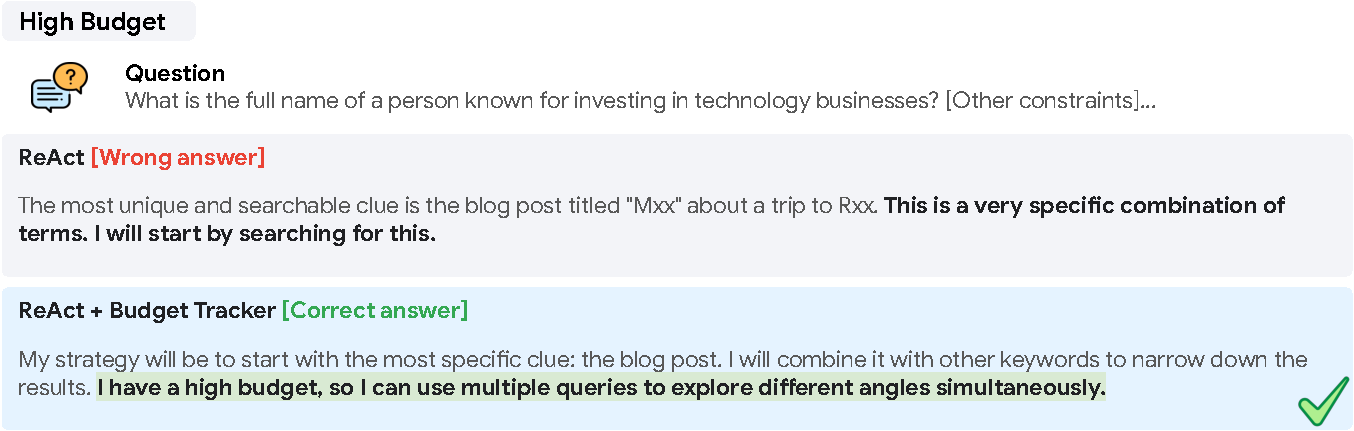
\includegraphics[width=0.95\linewidth]{assets/figs/case_high_bgt.pdf}
    \caption{Adaption to high budget constraints. Being aware of the high budget, the agent chooses to expand its search queries starting from a specific keyword, whereas ReAct immediately applies narrow conditions and fails.}
    \label{fig:case_high_bgt}
\end{figure}

\begin{figure}[htbp]
    \centering
    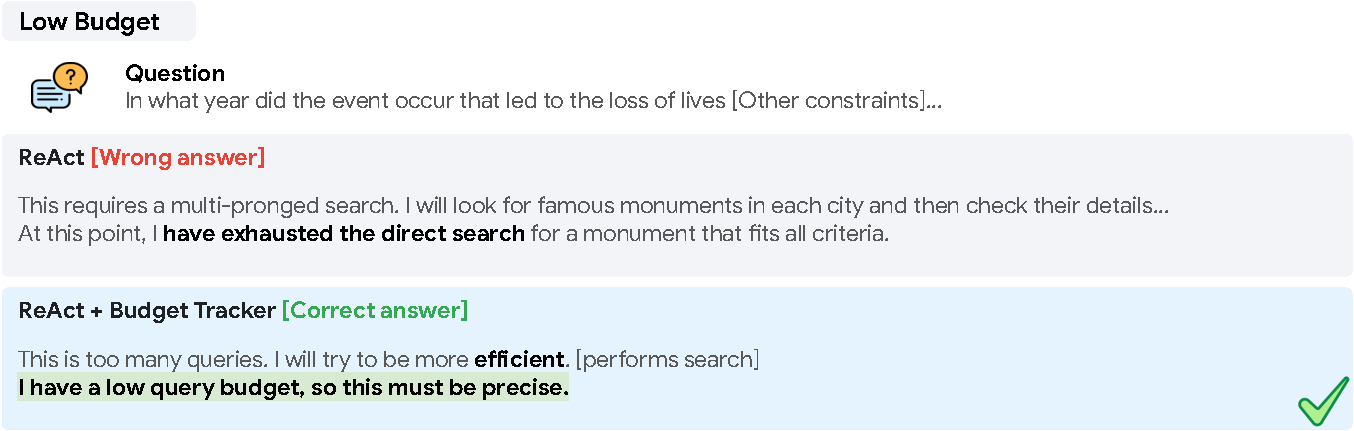
\includegraphics[width=0.95\linewidth]{assets/figs/case_low_bgt.pdf}
    \caption{Adaption to low budget constraints. Under a low budget, ReAct fails due to an exhaustive search strategy. In contrast, budget tracker helps the agent adapt by prioritizing query efficiency and precision, successfully solving the task.}
    \label{fig:case_low_bgt}
\end{figure}

\subsection{Adaptive Verification}

In Figure~\ref{fig:case_verification}, we demonstrate how self-verification module makes budget aware decision based on the trajectory and the resource status. It decides to pivot from the current pass because the remaining budget still allows for further investigation. These cases are collected from Gemini-2.5-Pro trajectories on BrowseComp.

\begin{figure}[htbp]
    \centering
    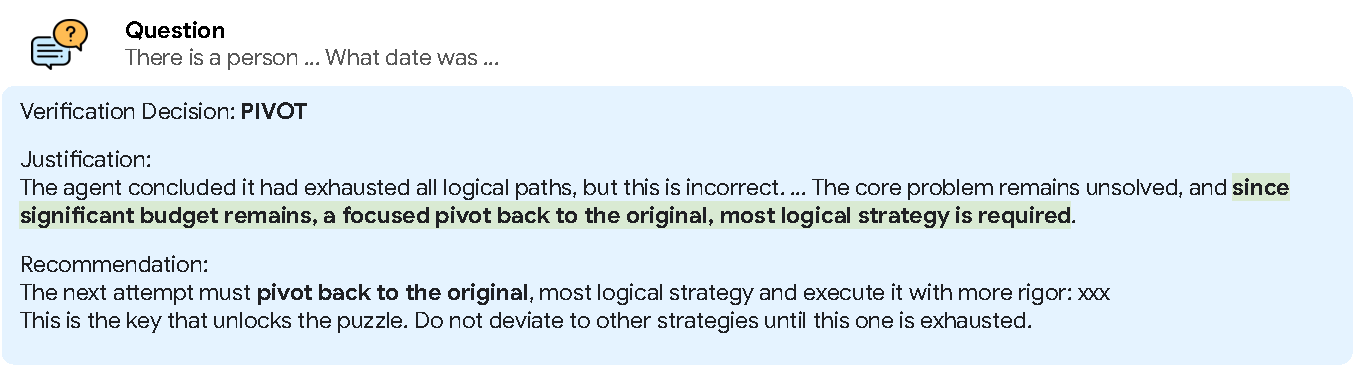
\includegraphics[width=0.95\linewidth]{assets/figs/case_verification.pdf}
    \caption{In \method, the verification process dynamically adapts to budget constraints. It successfully identifies the cause of failure and provides strategic recommendations based on the current trajectory. Following this advice allows the agents to better utilize the budget and arrive at the correct answer in the next attempt.}
    \label{fig:case_verification}
\end{figure}


\section{Limitations}


\textbf{More resource constraints.}
While our study presents the first empirical analysis of tool-call budgets, a more realistic and challenging scenario involves managing multiple resource constraints jointly. Examples include token limits, inference latency, and tool-call budgets. Understanding and controlling agent behavior under multi-dimensional constraints is important for deploying scalable systems in real environments.

\textbf{Resource allocation.}
Although we observe that budget awareness enables more effective scaling, we do not explore how an agent should allocate its available resources. Our empirical analysis suggests that models often underestimate their actual resource consumption, which can lead to suboptimal performance. Developing accurate resource estimation and principled budget allocation strategies is a promising direction for future work.

\textbf{More intelligent context management.}
Although we adopt several simple context control techniques such as removing tool responses and summarizing intermediate trajectories, more advanced context engineering remains largely unexplored. Designing more effective memory formats and identifying the right balance between context length and performance are important open challenges for building robust and efficient agents.
